\documentclass[10pt,twocolumn,letterpaper]{article}

\usepackage{cvpr}
\usepackage{times}
\usepackage{epsfig}
\usepackage{graphicx}
\usepackage{amsmath}
\usepackage{amssymb}
\usepackage{float}
\usepackage{subcaption}
\usepackage{placeins}
\usepackage{caption}
\usepackage{enumitem}
\let\vec\mathbf
\usepackage{etoolbox}
\patchcmd{\thebibliography}{\section*{\refname}}{}{}{}
\newcommand{\code}{\textit}
% Include other packages here, before hyperref.

% If you comment hyperref and then uncomment it, you should delete
% egpaper.aux before re-running latex.  (Or just hit 'q' on the first latex
% run, let it finish, and you should be clear).
\usepackage[breaklinks=true,bookmarks=false]{hyperref}

\cvprfinalcopy % *** Uncomment this line for the final submission

\def\cvprPaperID{****} % *** Enter the  Paper ID here
\def\httilde{\mbox{\tt\raisebox{-.5ex}{\symbol{126}}}}
\graphicspath{{figures/}}


% Pages are numbered in submission mode, and unnumbered in camera-ready
\setcounter{page}{1}
\begin{document}


%%%%%%%%% TITLE
\title{Grandad's Story - Stan Still}
\maketitle

\tableofcontents
\clearpage


%%%%%%%%% BODY TEXT
\subparagraph{Blurb}
The story of my grandad, Stanley Still.

\section{30/09/1930 - Pre-fostering}
\label{section:empirical_analysis}

\section{??/03/1932 - Fostered childhood}
\begin{itemize}
    \item Born
    \item Knows very little.
\end{itemize}

\section{??/06/1944 - Leaves School}
\begin{itemize}
    \item Leaves school on the Friday
    \item Starts work on the Monday at a bakery
    \item Mainly works on doing confectionaries 
    \item The bakery was in Chippin Norton
    \item He used to cycle
    \item Made his bike himself by finding a frame and some wheels from down the pit
    \item The back wheel was bigger then the front
    \item When it snowed he would pick up the bike and cover it over his shoulder
    \item They were still rationed so they couldn't really make much, they used "telefat" which was really solid so they used to have to soften it in hot water.
    \item He used to be quite good at icing cakes
    \begin{itemize}
        \item Used to cycle 5 miles every mile to Chippin Norton every morning
        \item Had to be there at 7am
        \item There was a big hill on the way so if it was snowing he'd have to pick the bike up and carry it
        \item When he turned 18 he had to leave the bakery because he got called up for his national service.
    \end{itemize}
    \item The woman who fostered him used to clean school
    \begin{itemize}
        \item So on the way to work he had to stop at the school and make sure that the fire was working ok
        \item Then he had to pump the water up into the tank, then it would pump around the school as central heating
    \end{itemize}
    \item At this time Vic was in the merchant navy
    \begin{itemize}
        \item Vic joined the merchant navy at 15
        \item He was 18 months older than Grandad
        \item Before he joined the merchant navy he went to work on a farm for a year.
        \item It was a mixed farm, used to have milking cows, and grew wheat, barley and oats.
        \item Most farms did very similar.
        \item You'd start with the barley, then the oats, then the wheat on a rotation
        \item It was all done manually, and a horse would pull a thing called a "binder" (havest binder), which makes wheat sheafs.
        \item After the binder had been through the children follow the binder and stand up the wheat sheafs and balance them so they were stood up so that they'd dry.
        \item After he left the farm he used to work part time for a Russian who Kossac riding (acrobatic) riding
        \item Vic wanted to go off with him touring
        \item But his foster mother wouldn't let him go because he would be used as a slave.
        \item Vic went in the Merchant navy when he was 15
        \item He got married when he was 17
        \item They had three daughters, called: Valerie and then two others who live in Chicago.
        \item Vic's wife was called Marie.
        \item 
        \item Valeries is the one who he goes to visit in Oxford.
        \begin{itemize}
            \item The other two married two Americans who were stationed at an airbase near Oxford.
            \item They met them in Oxford.
            \item And then they married both of them and went back to America after the war.
            \item This was ~18 years after the war.
            \item All three daughters were born in Kingham and then moved to Oxford.
            \item Valerie married an English bloke so she stayed.
        \end{itemize}
        \item He joine the merchant navy when he was 15
        \item He was in there for two years.
        \item Then when he came out he had to go and do his national service.
        \item He then went back into the merchant navy for another year or so (post marriage)
        \item Marie wanted him to come out of the merchant navy because she had three daughters under 5.
        \item Because every time he came back from the navy, she gets pregnant.
        \item Then they move to Oxford because he got a job in a car factory.
        \item He then works in that car factory for the rest of his working life (~30-65)
    \end{itemize}
    \item At this point Grandad did not even know that he had an older brother. 
    \begin{itemize}
        \item He first met Ron when he was about 17.
        \item Ron was 4 years older than Stan.
        \item He was living in Guildford.
        \item He knew the address somehow, presumably from when they were fostered.
        \item He wrote a letter telling them that he was coming down
        \item Then they met him off the train.
        \item He doesn't know if his foster mum knew he had an older brother, but he doubts it.
        \item But she was fine with him coming to meet them.
        \item By this point Ron had got married and that was why he was living Guildford.
        \item Grandad's dad was also living in Guildford.
        \item But his dad didn't come to visit.
        \item Grandad never met his dad.
        \begin{itemize}
            \item Grandad assumes that Ron grew up in East London, but he didn't sound like a cockney.
            \item Then he moves to Guildford with his dad at some point.
            \item Grandad doesn't really know what he did when left school.
            \item He was in the RAF during the war and he was an Airgunner.
            \item After the war he worked somewhere to do with the testing of concord.
            \item (Concord was being built at Bristol, then it moved to Fairford for testing) This was near Grandad so this is the bit he knows about.
        \end{itemize}
    \end{itemize}
    \item The first that he really knew about his dad was when he was in the RAF.
    \begin{itemize}
        \item So when he was on his 48 hours off of leave.
        \item And so one day when he was visiting her aunty his Dad rang the house phone.
        \item So his dad said that he'd like to meet up.
        \item When he hangs up his aunty says that "you don't want anything to do with him"
        \item So when he gets back to camp he writes a letter to his dad saying that he doesn't see the point in meeting up, because he's a  stranger, and when Grandad needed him he wasn't there, so he didn't want to meet him.
    \end{itemize}
    \item He had an aunty in Sreatham
    \begin{itemize}
        \item Grandad said "she was a gay old bird".
        \item She used to be a dancer on the stage.
        \item She was a chorus girl or something like that.
        \item And she lived with this bloke, basically as a mistress.
        \item She was kind of like his kept woman.
        \item This guy was quite well off, but he wouldn't marry her.
        \item But his two sons made sure that he never married her.
        \item She used to drink a lot.
        \item Whenever Grandad went down the first thing they'd do was go straight to the pub.
        \item Her name was Ada, and everyone knew here in the pub so she drank a lot.
        \item In the end she ended up in a mental home.
        \item After Grandad was married to Whinney, police came and knocked on the door one night and said: "Do you know an Ada Still" and he said "Yes" and they said she's been taken into a hospital in Balham because she had tried to take an overdose.
        \item Then later they communicated to Grandad that she'd been taken to a mental hospital down in Surrey somewhere.
        \item So Grandad and Whinney went and saw in the place in Surrey.
        \item She did not seem alright at all, she seemed fully out of her mind.
        \item She really wanted matches. Presumably to burn either herself or the home.
        \item The only way that they could get away from her was by telling her that they were going out to get some matches.
    \end{itemize}
    \item Grandad also had an uncle called Arthur
    \begin{itemize}
        \item Arthur lived in New York
        \item He worked in the hotel business.
        \item When he retired he came over to see Grandad and Whinney.
        \item They were living in rooms (~1952/53) in Cirencester.
        \item Vic was living in Kingham.
        \item Grandad used to have a moterbike, and you took Arthur to Kingham to introduce him to Vic.
    \end{itemize}
\end{itemize}


\section{~Work pre national service}

\section{30/09/1948 - National service}
\begin{itemize}
    \item He got called up when he turned 18, because everyone had to do their national service.
    \item The first 8 weeks you go to a camp and they give you a uniform
    \item You spend the first 8 weeks doing "square bashing" (marching/drill) and learning to shoot a rifle
    \item After 8 weeks they got sent to a new camp, (Insworth in Gloucester)
    \item Because he'd been a baker he got sent to the catering one (quatermaster)
    \item When he finished the 8 week cookery course he got posted at Watton in Norwich
    \item Watton was a general camp, a flying station.
    \item There three messes, the airman's mess, the sergeant's mess and the officer's mess.
    \item Everyone started in the airman's mess, then if you were and good and lucky then you could get pulled up into the officer's mess.
    \item 
    \item Went to a training camp somewhere 
    \begin{itemize}
        \item One night he was the duty cook
        \item Thank meant that he had to be there until about 8pm at night. 
        \item He put meat in for about 400 men
        \item And then he forgot, he should have taken it out when he went off duty at 10pm.
        \item There was some guy who looked after the boilers, and he came over to Grandad's quaters.
        \item This guy came over and shook him, Grandad was asleep.
        \item asks if Grandad is the duty cook,
        \item Grandad say's he is 
        \item He says you left it in 
        \item And when you went and checked it was about a quater of the size it should be and very burnt.
        \item So he didn't sleep much that night.
        \item So Stan went and had a worked in a guy who he knew in the stores. 
        \item He gave him two joints of the officers meat.
        \item This was all at about 8am in the morning.
        \item So Stan slipped them into the oven.
        \item So the sergeant asked him why he was cooking stuff at 8am. 
        \item And Stand lies and says that he left two of them in the stores by mistake.
        \item So he Stan had to slice the meat really thin
        \item He said that the beef was that hin that he was worried it might dissolve in the gravy.
        \item But he got away with it
    \end{itemize}
    \item On a Saturday night they used to go from Watton to Norwich
    \begin{itemize}
        \item Norwich used to put on a dance at Norwich town hall.
        \item One night Stan went and he met this girl, and he was dancing with this girl.
        \item In those days you were always expected to walk a girl home.
        \item But the girl about 2 miles away from the hall
        \item The lorry used to leave between 10pm and 10:15 to take them back to camp.
        \item By the time he got back to Norwich Town hall the lorry had gone.
        \item So then he knew that the only way he could get back to camp was by walking.
        \item He'd been walking for he doesn't know how many miles he'd been walking for, but it was baout 20 miles from Norwick to Watton camp.
        \item So after a while, he saw this horse.
        \item He tried to catch it, he was going to try and run it back to camp.
        \item But every time he got it to near a wall so that he could jump on, but every time he tried it would run away.
        \item He started to walk again, but then luckily some guy in car came along, and asked where he was going, then he gave him a lift to within about a mile of the camp.
        \item Then he walked back from there.
        \item He made it back just in time. 
        \item He made it back just in time for 6:30am.
    \end{itemize}
    \item He made friends with people because you're all sleeping in the same place basically on top of each other.
    \item Also you're working the same shifts so you get to know each other.
    \item So because they were good firends they'd all socialise together and they'd go out drinking together if they had enough money.
    \item Beer was only about 4pence or 6pence in those days.
    \item He didn't stay in touch with any of them afterwards.
    \item The only time he saw a couple of them was when he had to do H-reserve.
    \item You had to go back to some random camp for two week every year.
    \item He only had to go one year because he was working at the agricultural college in Cirencester and the burser (head of the college) managed to get him out of it every year but one.
    \item Stan had to go to a place just outside Southampton.
    \item Stan had to go but head
    \item When you finished your national service, you got to keep your kit, so he hadn't seen it since he was in it.
    \item It properly smelled.
    \item One guy he met had used his trousers for working as a fireman on the railway, so his trousers were filthy.
    \item When he got to the camp in Southampton, they couldn't believe it. The people at the camp hadn't heard anything about them so they didn't know they were coming.
    \item The first thing they did was take them to the stores and give them all new uniforms.
    \item When he finished with the RAF, he went back to the abker in Chippin Norton.
    \item At that time they were making it more mechanised.
    \item So jobs were dissapearing, but Grandad was doing all the puff pastry and icing cakes, and the layborough who was greasing tins was getting more money than Stan.
    \item So Stan went to the office and said that this is taking the piss.
    \item And they said that we can't pay you a mans wage because you're not 21 yet.
    \item So he said you can keep the job.
    \item So he went and got a job down at Kingham Hall school.
    \item He got a job as an under-chef/assistant-chef.
    \begin{itemize}
        \item With milk
        \item Without milk
    \end{itemize}
    \item He was working at a flying base 
    \item He used to have to put the food in for the pilots the night before at about midnight
    \begin{itemize}
        \item He put in the 
        \item Without milk
    \end{itemize}
    \item But one day he did it and 
\end{itemize}

\section{Post national service}
\begin{itemize}
    \item Come out of the RAF and went back to the bakery in Chippin Norton
    \begin{itemize}
        \item The people who were greasing tins were getting paid more than he was
        \item He said this it taking the piss
        \item And they said that they couldn't pay him a mans wage so he said they could keep their job
    \end{itemize}
    \item Was working as an assistant chef at Kingham Hall School
    \item He was there for about 18 months
    \item It was ok.
    \item He was having to live with his sister because the woman who brought him up had married again and her new husband didn't want Stan around.
    \item So one of the big attractions of this job was that it had free accomodation.
    \item His sister was still living in Kingham, and she lived there all her life.
    \item His sister was married with a young baby.
    \item It wasn't very convenient living with his sister because they only had a small cottage with one bedroom and one up in the loft.
    \item So he goes to this boarding school near Birkhampstead
    \item So you went up for interview, and then he got the job. 
    \item He was living in accomodation at the school.
    \item He was friendly with the rest of the staff.
    \item Whinney was one of about 6 waitresses.
    \item There were people who peeled potatoes, (Kitchen porters), a veg cook, a woman who did all the deserts.
    \item It was quite a big school. There were boys and girls, they were separated, boys on one side of the school, girls on the other. 
    \item He met Nana there
    \begin{itemize}
        \item She was a waitress in the dining room, giving the children food at each meal time.
        \item After a while Stan asked Nana if she'd like to go to the pictures.
        \item So they went to the cinema.
        \item So most weekends they went to the cinema
        \item Sometimes they got a meal or something.
    \end{itemize}
    \item There weren't that many people worth mentioning.
    \item You were just one of a crowd, everyone had their own job. 
    \begin{itemize}
        \item He met Nana there
        \item Learned more about cooking there
        \item There was this women there who he couldn't get on with
        \item He used to get this cooking journal, and he saw an advert for beign a chef at the royal agricultural college in Cirencester.
        \item He got the job so he ended up there
    \end{itemize}
    \item One day he nearly burnt the place down
    \begin{itemize}
        \item They used to cook for the children and all the teachers seperately
        \item He was cooking chips
        \item He'd just put the chips in so he went up for a shower
        \item He was over the other side in the same block of acoomodation as the girls
        \item The local guy who did the boilers saw the flames in the glass dome 
        \item Grandad comes back and the boiler man has manged to put it out.
        \item Grandad said that the guy looked like he'd sprayed the fire extinguished basically everywhere but the fire, but he had got it under control
        \item If that guy hadn't seen then the school would probably have burnt down
        \item Also Grandad had handed in his notice so he was worried that he could end up doing time becuase they might think he'd done it deliberately
    \end{itemize}
    \item Moving on
    \begin{itemize}
        \item There was this women there who he couldn't get on with
        \item She was a housekeeper, she was in charge of all the domestic  women, cleaners and stuff like that.
        \item She wasn't his boss, but she thought she could do anything she liked.
        \item She moved him to a room that he didn't like which was right on top of the swimming pool
        \item So all the noise and smell came up into the room
        \item So Grandad told her what she could do with his room
        \item So the next thing he knows the headmaster has sent ofr him.
        \item So the moment he goes in he doesn't give the HM a chance to say anything
        \item He says that he's breaking the terms of his contract and that in there it says he shoudl have appropriate accomodation, and this isnt.
        \item He said that she could shove her room where the monkey sticks his nuts.
        \item He was always looking for jobs.
        \item He used to get this cooking journal, and he saw an advert for beign a chef at the royal agricultural college in Cirencester.
        \item He got the job so he ended up there.
        \item By the time this fight happened he'd already written to the other place, been for an interview and got the job in Cirencester.
        \item This was why you were particularly worried they'd thigk it was deliberate.
    \end{itemize}
    \item So Grandad moves to Cirencester for the job at the RAC.
    \begin{itemize}
        \item The job provided accomodation.
        \item The manager was a really nice guy
        \item When Stan went there he told the boss that he was courting Nana in Birkhampstead.
        \item So the boss said that every month he could have the Firday offa nd have a long weekend to go and see Nana in Birkhampstead.
        \item It's over 100 miles between the two.
        \item So Stan had to get a train from Ciren to London, a train from London to Watford and then a bus from Watford to Birkhampstead.
        \item Stan worked at the RAC until he got married and then after that.
        \item So Stan Nana if she wanted to get married and she agreed.
        \item At that point she was still working in Birkhampstead.
        \item They fixed a date for the wedding and Stan went up to see her Dad to ask him if it was alright.
        \item Stan says that she was one of 5 sisters and he was probably glad to get rid of here (joke).
        \item This was the first time he'd met her dad.
        \item They went up for a long weekend to stay with her parents and that was when he ahd to ask him.
        \item He most of her family at that point. He met all her other sisters because they all lived in Seham anyway.
        \item They got married in Seaham.
        \item Stan asked her where she wanted to live, Birkhampstead, Seaham or Cirencester, and she said she wanted to come to Cirencester, so they did. 
        \item They got married in a catholic church because Nana was a catholic.
        \item They went to blackpool for their honey moon. 
        \item They had blackpool pier
        \item They had a big dance in a big ball room. (Blackpool tower ball room)
        \item They would go dancing and go on the funfair, and spend time on the beach.
        \item Their honeymoon was 1 week.
        \item They couldn't afford any more.
        \item When they decided to get married and they were going to move to Cirencester.
        \item They couldn't find any houses because they couldn't afford one and also you needed to be on the waiting list for about 2 years before you got one (council house).
        \item They were renting a room out from an old lady.
        \item They had the use of the front room, bedroom and sharing the kitchen.
        \item This was in Cirencester, about 1 mile away from work.
        \item Nana wasn't allowed to live at the place he'd been living before (they had to find new digs)
        \item Grandad found this new place (the old lady) in the news paper.
        \item So he found his first two jobs and his first house in the news paper.
        \item You used to have all the deaths, marriages etc and rooms in the local paper.
        \item They live in that house for about 2 years.
        \item He's still working at the RAC that whole time.
    \end{itemize}
    \item After that time they managed to rent a small cottage
    \begin{itemize}
        \item It was a small cottage
        \item It was 1 down and 2 up.
        \item A living downstairs with a kitchen
        \item Then there were two bedrooms upstairs, one bedroom and one attic.
        \item The attic was above the bedroom (3 storied)
        \item They used the attica s a spare room in case anyone came to stay. (eg her sisters)
        \item They lived in that cottage for about two years
    \end{itemize}
    \item Grandad was working on the busses at this point
    \begin{itemize}
        \item At this point Grandad was working on the busses down in Cirencester as a conductor
        \item He did that for about 18 months
        \item He left the RAC because he got fed up of working weekends when Nana was off. 
        \item So that meant that he didn't have any time off with Nana.
        \item They used to open it up in the summer for courses so he worked all year round.
        \item 
    \end{itemize}
    \item When they were living in the cottage the lady next door's dad had a removals business, they hauled coal and also furniture.
    \item One night he'd come round and they were talking, and Nana's family had wanted her to move back up north ebcause they didn't like her being so far away.
    \item The guy said "Are you serious about going up the north, because I've got a guy who wants to move up to newcastle and doesn't have much stuff, so if you had your stuff as well it would make it worth while"
    \item When they were living in the cottage Nana worked as a waitress in a restaurant. 
    \item While they were living in that cottage Nana had Paul (insert date here)
    \item So they talked it over that night (moving)
    \item Grandad thought it would be better because all of Nana's three sisters and family (big irish) lived up the north and so it would be  better for paul because he'd have cousiins and family tog row up around.
    \item They decided all in that one night.
    \item So then they moved up two or three weeks after.
    \item 


\end{itemize}


\section{Living up the north (Paul is 18 months)}
\begin{itemize}
    \item So they moved up there
    \item But Grandad couldn't goet a job down the mines
    \item Nana's dad had kept saying, come up here, I'll get you a good job down the mines.
    \item Grandad never went down a mine because he couldn't get a job.
    \item They didn't want a southerner down the pit
    \item Those jobs were passed down father to son,
    \item In retrospect was pleased that he didn't go down the mines because of the conditions that they worked in and breathing in all the dust and the health conditions
    \item Also he avoided the carnage of Thatcher 
    \item Jobs were hard to come-by because everyone worked down the pit
    \item So you saw an advert in the paper about going door to door selling vacuum cleaners.
    \item And you thought you'd give it a go because he had nothing else
    \item They were told to go in and start hoovering the carpet.
    \item And you'd hoover one section, then you'd dump the dirt on the carpet so that they could see the dirt and see why they needed a new hoover.
    \item And they also were supposed to sell this thing that sprayed water which you could use for paiting and cleaning your carpet and stuff.
    \item So in one ladies house, Grandad spent about 90 mins in there, and hoovered all the down stairs carpet, and then she said she didn't want it.
    \item He kept going because it was showing how good it was.
    \item But then she said she didn't want it, so he turned the hoover round and used the blowing end to blow the dirt all over her.
    \item So she said "ypu'd blown dirt all over me", and he said, "Well it's your dirt Mrs" and then scarpered.
    \item Grandad was a hoover salesman for about 9 months.
    \item He was that fed up after 9 months (about when the lady incident happened) that he went back to the centre and said you can keep your job.
    \item He then went and got a job on the busses up the north
    \item It was alright, but he wasn't happy doing it, he'd already left the busses down in Cirencester because he was fed up with it, but it was the only job he could find, so he just had to put up with it.
    \item When people would get on they'd tell him where tehy wre going, and he was supposed to ring the bell when they got to that stop, but he couldn't rememebr all the stops, so they'd go mad if he didn't ring it.
    \item Also people had really strong geordie accents so he coudlnt' understand what they were saying, "It was like working in a foreign country"
    \item When grandad worked on the busses, when they came in, if you were on the night shift then you'd all go back to depo and then you'd have to wait for all the other busses to come in to give you a lift home.
    \item So they'd be waiting for and hour or so so they'd play cards.
    \item One night grandad went in and they were playing 3 card brag. 
    \item Every round everyone puts in a six pence or whatever you wre playing for.
    \item And so at the start htere were lots of people 5/6
    \item Then as you're playing if people are doing badly they "pack their hand", drop out.
    \item Grandad was one of the last two playing, so he got to the end and this guy kept bragging, but Grandad had three threes, which was the highest hand that you could have in brag.
    \item So they got to the end, the guys said "I'll see you then" and he had a Jack, Queen, King, which was a good hand. 
    \item And the guy got annoyed because he was saying that "Grandad should have declared that he'd got that hand at the start, but Grandad said, no one told me any rules when I sat down so I didn't know, and he took the money"
    \item At the time they were living with Nana's mum and dad.
    \item Nana's dad used to drink a lot, he would drink a lot in the morning
    \item Because he'd had four daughters they'd always have to do what he said. Because he'd never had a son no-one ever challenged him.
    \item One night Grandad came in from work.
    \item And her dad would come in from work and pull a drink
    \item When he was drunk was the time he'd talk
    \item Whenever he came in his wife always had to make him dinner.
    \item So he came in drunk and his wife made him food as per.And then he said to Grandad "Come up and get somethign to eat" and Grandad said, "I'm alright, I've already eaten", and then one thing led to another and he started saying "Do you think you're a better man than me", and Grandad said "No I don't think I'm a better man than you, but I'm as good until you show me different". Then they nearly came to blows, and his wife was crying and Nana was upset but it all blew over.
    \item But from then Grandad knew that he didn't want to live there because feel comfortable.
    \item And every weekend when he was drunk you'd have to sit there and listen to him, you'd think from what he said that "Him and the yanks won the war"
    \item Nana's dad did fight in the war, but he wasn't in a fighting unit, he was in the pioneering corps because he only had one eye.
    \item He lost his other eye because in his younger days he went to work in Canada and that's where he lost his eye.
    \item He was born and bred in Seaham 
    \item He married Nana's mum when he came back
    \item When grandad wasn't working he'd go to the working men's club during the week. There were four or five working men's clubs for miners in Seaham harbour, he used to go out with the other son in laws. 
    \item At this point all of Nana's sisters were married, apart from Rose. 
    \item He normally went out with the other son in laws.
    \item Every Saturday they used to have dances at one of the working men's clubs, so they would all go down.
    \item Women were only allowed upstairs, they weren't allowed in the bars. they were only allowed in the "Lounge".
    \item It sounds weird to me now, and it seemed weird to Grandad then. Because women were allowed in pubs in the south, but they weren't allowed in the North.
    \item The reason women weren't allowed in the bar was that it meant men didn't have to mind their language and so they could eff and blind if they wanted to.
    \item Going up the north was really like being in a different country.
    \item But when they moved up there Rose was only about 3.
    \item Rose is only slightly older than Paul.
    \item It wasn't long after that Grandad went down the north.
\end{itemize}



\section{Pre car factory}

\section{Car factory}

\section{Paul's born}

\section{Michelle's born}

\section{Car factory}



\clearpage

\section{}
\subsection{Data Flows and Dependencies}

\begin{figure*}
    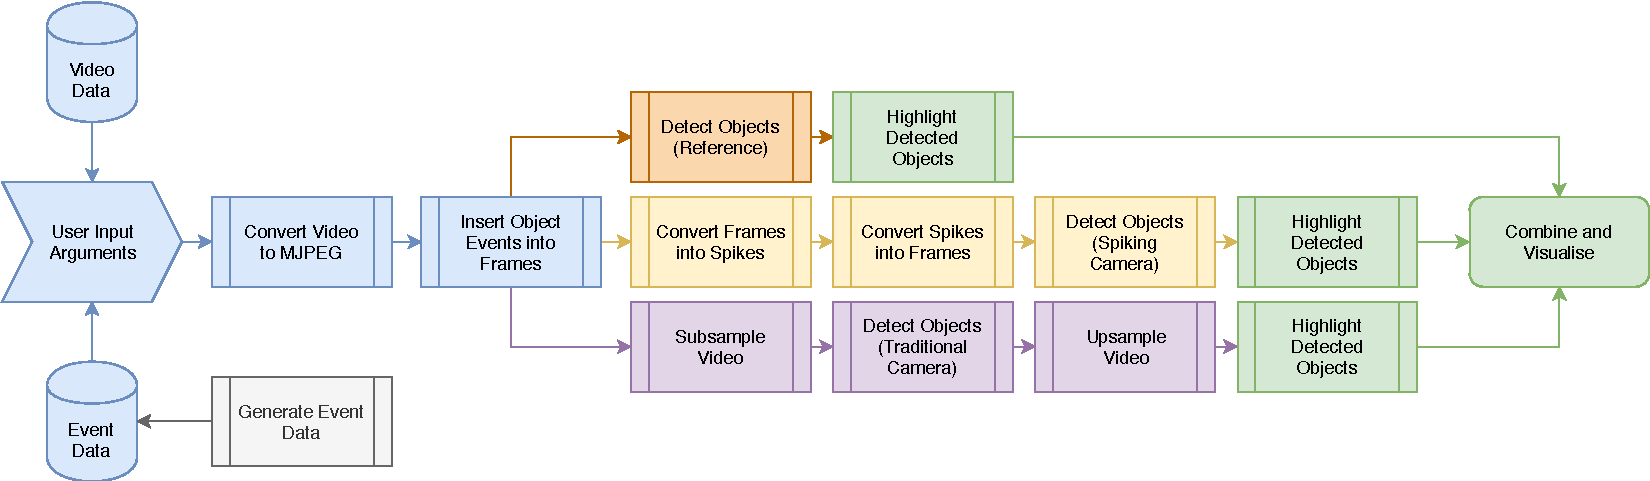
\includegraphics[width=\textwidth]{process_diagram}
    \caption{A representation of the complete program flow and the data dependencies.}
    \label{fig:process_diagram}
\end{figure*}

The flow of data and its dependencies throughout the application is shown in Figure \ref{fig:process_diagram}. In the ideal case of maximum pipelining efficiency, each process block would continuously output data. The basic implementation of the application in \code{standard\_flow.sh} runs each step in serial and outputs the result to a file before continuing, thus there is overhead in writing to disk and a complete lack of pipelining.

\subsection{Complexity Analysis \& Bottlenecks}
\label{section:complexity_analysis}
\begin{table}
    \captionsetup{singlelinecheck=off}
    \begin{center}
    \resizebox{\linewidth}{!}{
    \begin{tabular}{l|c|c}
    \textbf{Program} & \textbf{Asymptotic Complexity} & \textbf{\% of Execution Time} \\
    \hline
    \code{frame\_to\_object\_stream} & $\mathcal{O}(f*e*\log{e})$ & 95.18 \\
    \code{frame\_to\_spikes} & $\mathcal{O}(f * (h*w + c*\log{c}))$ & 2.33 \\
    \code{spikes\_to\_frame} &  $\mathcal{O}(f)$ & 0.99 \\
    \code{frame\_insert\_objects} & $\mathcal{O}(f*e_{pf}*w_{p}*h_{p}*scale^2)$ & 0.98 \\
    \code{frame\_subsample} & $\mathcal{O}(f*h*w)$ & 0.52 \\
    \code{object\_stream\_stretch} & $\mathcal{O}(f*e_{pf}*o)$ & 0.00 \\
    \code{frame\_highlight\_objects} & $\mathcal{O}(f*e_{pf}*scale)$ & * \\
    \code{generate\_object\_stream} & $\mathcal{O}(f)$ & * \\
    \end{tabular}
    }
    \end{center}
    \caption[]{
        The complexities of the original code. Definitions:
    \begin{align*}  
        f &= \text{number of frames}\\
        c &= \text{number of candidate spikes}\\
        h*w &= 720*1280 = 9.2e6 \: \text{pixels (See Section \ref{sec:CurrentBottlenecks})}\\
        e &= \text{number of potential events during classification}\\
        e_{pf} &= \text{number of events per frame}\\
        o &= \text{oversampling factor} \\
        w_{p}, h_{p} &= \text{Width and height of the pattern}
    \end{align*}
    *Steps run as part of the initialisation/visualisation, not considered part of the critical application.
    }
    \label{table:complexity}
\end{table}

The original complexities of the programs called from \code{standard\_flow.sh} are shown in Table \ref{table:complexity}. The majority of the total execution time is spent executing \code{frame\_to\_object\_stream} and within this program, the sorting of the events (of complexity $e\log{e}$) dominates.

\nocite{*}

%-------------------------------------------------------------------------
% \newpage
{
 \small
 \bibliographystyle{ieee}
 \bibliography{bibliography}
}
\end{document}
